\documentclass[tikz]{standalone}

\usepackage{tikz}
\usepackage{pgfplots}
\usetikzlibrary{matrix, positioning, shapes}
\usetikzlibrary{arrows, automata, shadows, patterns}

\begin{document}
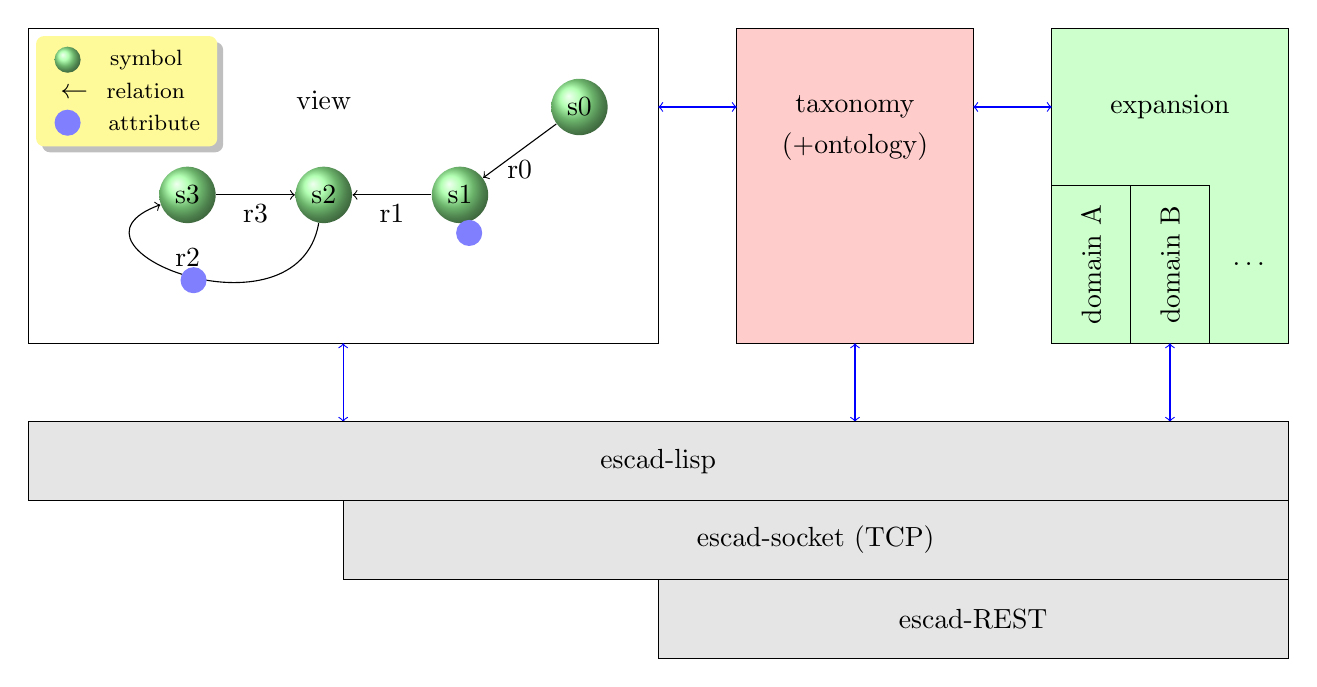
\begin{tikzpicture}[
      node distance=0.6cm and 1cm,
      sym/.style={circle, shading=ball, ball color=green!40, minimum size=0.5mm},
      atr/.style={circle, fill=blue!50, minimum size=0.5mm}]
    \node[sym] (s0) {s0};
    \node[sym] (s1) [below left=of s0] {s1};
    \node[atr] at (-1.4,-1.6) {}; % s1 attribute
    \node[sym] (s2) [left=of s1] {s2};
    \node[sym] (s3) [left=of s2] {s3};
    \draw[->] (s0) -- (s1) node [pos=0.5, below] {r0};
    \draw[->] (s1) -- (s2) node [midway, below] {r1};
    \draw[->,out=-100,in=200,looseness=2] (s2) to node[above,pos=0.5] {r2} (s3);
    \node[atr] at (-4.9,-2.2) {}; % r2 attribute
    \draw[->] (s3) -- (s2) node [pos=0.5, below] {r3};
    \draw[draw=black] (1,1) rectangle ++(-8,-4);
    \node[] (view) [above=of s2] {view};
    \draw[draw=black, fill=red!20] (2,1) rectangle ++(3,-4);
    \node[] at (3.5,0) {taxonomy};
    \node[] at (3.5,-0.5) {(+ontology)};
    \draw[draw=black, fill=green!20] (6,1) rectangle ++(3,-4);
    \node[] at (7.5,0) {expansion};
    \node[] at (8.5,-2) {$\dots$};
    \draw[draw=black] (6,-1) rectangle ++(1,-2);
    \node[rotate=90] at (6.5,-2) {domain A};
    \draw[draw=black] (7,-1) rectangle ++(1,-2);
    \node[rotate=90] at (7.5,-2) {domain B};
    \draw[<->,blue] (-3,-4) -- (-3,-3) node [pos=0.5] {};
    \draw[<->,blue] (3.5,-4) -- (3.5,-3) node [pos=0.5] {};
    \draw[<->,blue] (7.5,-4) -- (7.5,-3) node [pos=0.5] {};
    \draw[<->,blue] (1,0) -- (2,0) node [pos=0.5] {}; % view -tax
    \draw[<->,blue] (5,0) -- (6,0) node [pos=0.5] {}; % tax - exp
    \draw[draw=black, fill=black!10] (-7,-4) rectangle ++(16,-1);
    \node[] at (1,-4.5) {escad-lisp};
    \draw[draw=black, fill=black!10] (-3,-5) rectangle ++(12,-1);
    \node[] at (3,-5.5) {escad-socket (TCP)};
    \draw[draw=black, fill=black!10] (1,-6) rectangle ++(8,-1);
    \node[] at (5,-6.5) {escad-REST};
    % legend:
    \draw[draw=none, rounded corners=1mm, fill=yellow!40, drop shadow] (-6.9,0.9) rectangle ++(2.3,-1.4);
    \node[sym] at (-6.5,0.6) {};
    \node at (-5.5,0.6) {\footnotesize{symbol}};
    \node at (-5.8,0.2) {$\leftarrow$\ \ \footnotesize{relation}};
    \node[atr] at (-6.5,-0.2) {};
    \node at (-5.4,-0.2) {\footnotesize{attribute}};
\end{tikzpicture}

\end{document}